\begin{figure}
\centering
\begin{tikzpicture}
  \node (circ) {
    \begin{tikzpicture}
      \node[inner sep=0pt] (circuit) {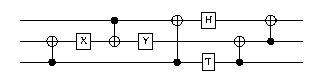
\includegraphics[scale=2, trim={2.5mm 0 2.5mm 0}, clip]{Figures/circuits/pullCirc}};  
      \node[left=-7mm of circuit.west, rectangle,fill=white,minimum height=22mm, minimum width=8mm] {};
      \node[right=-7mm of circuit.east, rectangle,fill=white,minimum height=22mm, minimum width=8mm] {};
      \node[above left=4.5mm and -7mm of circuit.west, opacity=0.9] {\footnotesize \(A\)};
      \node[left=-7mm of circuit.west, opacity=0.9] {\footnotesize \(B\)};
      \node[below left=4.5mm and -7mm of circuit.west, opacity=0.9] {\footnotesize \(C\)};
      \node[right=-3mm of circuit.north west, font=\itshape] (text) {a)};
    \end{tikzpicture}
  };
  \node[below=5mm of circ] (pulled) {
    \begin{tikzpicture}
      \node[inner sep=0pt] (circuit) {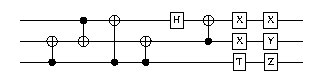
\includegraphics[scale=2, trim={2.5mm 0 2.5mm 0}, clip]{Figures/circuits/pullPulled}};  
      \node[left=-7mm of circuit.west, rectangle,fill=white,minimum height=22mm, minimum width=8mm] {};
      \node[right=-7mm of circuit.east, rectangle,fill=white,minimum height=22mm, minimum width=8mm] {};
      \node[above left=4.5mm and -7mm of circuit.west, opacity=0.9] {\footnotesize \(A\)};
      \node[left=-7mm of circuit.west, opacity=0.9] {\footnotesize \(B\)};
      \node[below left=4.5mm and -7mm of circuit.west, opacity=0.9] {\footnotesize \(C\)};
      \node[right=-3mm of circuit.north west, font=\itshape] (text) {c)};
    \end{tikzpicture}
  };
  \node[above right=-32.5mm and -2mm of circ] (hypergraph) {
    \begin{tikzpicture}
      \coordinate (O) at (0,0);
      \coordinate (A) at (90:12mm);
      \coordinate (B) at (210:12mm);
      \coordinate (C) at (330:12mm);
      \draw (O) -- (A);
      \draw (O) -- (B);
      \draw (O) -- (C);
      \draw (A) edge[out=210,in=90,looseness=1] (B); 
      \draw (A) -- (B);
      \draw (B) -- (C);
      \node[circle, right=-2.5mm of A, fill=white, inner sep=0pt, minimum size=5mm] {\(A\)};
      \node[circle, right=-2.5mm of B, fill=white, inner sep=0pt, minimum size=5mm] {\(B\)};
      \node[circle, right=-2.5mm of C, fill=white, inner sep=0pt, minimum size=5mm] {\(C\)};
      \coordinate (leftPoint) at (270:11.5mm);
      \coordinate (rightPoint) at (30:11.5mm);
      \pic (cut) {cut=leftPoint/rightPoint};
      \node[above left=0mm and 13mm of A, font=\itshape] (text) {b)};
    \end{tikzpicture}
  };
  \node[above right=-32.5mm and -2mm of pulled] (hypergraph2) {
    \begin{tikzpicture}
      \coordinate (O) at (0,0);
      \coordinate (A) at (90:12mm);
      \coordinate (B) at (210:12mm);
      \coordinate (C) at (330:12mm);
      \draw (O) -- (A);
      \draw (O) -- (B);
      \draw (O) -- (C);
      \draw (A) edge[out=210,in=90,looseness=1] (B); 
      \draw (A) -- (B);
      \node[circle, right=-2.5mm of A, fill=white, inner sep=0pt, minimum size=5mm] {\(A\)};
      \node[circle, right=-2.5mm of B, fill=white, inner sep=0pt, minimum size=5mm] {\(B\)};
      \node[circle, right=-2.5mm of C, fill=white, inner sep=0pt, minimum size=5mm] {\(C\)};
      \coordinate (leftPoint) at (270:11.5mm);
      \coordinate (rightPoint) at (30:11.5mm);
      \pic (cut) {cut=leftPoint/rightPoint};
      \node[above left=0mm and 13mm of A, font=\itshape] (text) {d)};
    \end{tikzpicture}
  };
\end{tikzpicture}
\vspace*{5mm}
\caption{Example where an ebit can be saved by sliding CNOTs closer together. This figure shows the original circuit \textit{a)}, its optimally partitioned hypergraph \textit{b)}, the pre-processed circuit \textit{c)}, and its optimally partitioned hypergraph \textit{d)}, which has one less cut hyperedge.}
\label{fig:pulledCNOTexample}
\end{figure}